

%% bare_conf.tex
%% V1.4
%% 2012/12/27
%% by Michael Shell
%% See:
%% http://www.michaelshell.org/
%% for current contact information.
%%
%% This is a skeleton file demonstrating the use of IEEEtran.cls
%% (requires IEEEtran.cls version 1.8 or later) with an IEEE conference paper.
%%
%% Support sites:
%% http://www.michaelshell.org/tex/ieeetran/
%% http://www.ctan.org/tex-archive/macros/latex/contrib/IEEEtran/
%% and
%% http://www.ieee.org/

%%*************************************************************************
%% Legal Notice:
%% This code is offered as-is without any warranty either expressed or
%% implied; without even the implied warranty of MERCHANTABILITY or
%% FITNESS FOR A PARTICULAR PURPOSE! 
%% User assumes all risk.
%% In no event shall IEEE or any contributor to this code be liable for
%% any damages or losses, including, but not limited to, incidental,
%% consequential, or any other damages, resulting from the use or misuse
%% of any information contained here.
%%
%% All comments are the opinions of their respective authors and are not
%% necessarily endorsed by the IEEE.
%%
%% This work is distributed under the LaTeX Project Public License (LPPL)
%% ( http://www.latex-project.org/ ) version 1.3, and may be freely used,
%% distributed and modified. A copy of the LPPL, version 1.3, is included
%% in the base LaTeX documentation of all distributions of LaTeX released
%% 2003/12/01 or later.
%% Retain all contribution notices and credits.
%% ** Modified files should be clearly indicated as such, including  **
%% ** renaming them and changing author support contact information. **
%%
%% File list of work: IEEEtran.cls, IEEEtran_HOWTO.pdf, bare_adv.tex,
%%                    bare_conf.tex, bare_jrnl.tex, bare_jrnl_compsoc.tex,
%%                    bare_jrnl_transmag.tex
%%*************************************************************************

% *** Authors should verify (and, if needed, correct) their LaTeX system  ***
% *** with the testflow diagnostic prior to trusting their LaTeX platform ***
% *** with production work. IEEE's font choices can trigger bugs that do  ***
% *** not appear when using other class files.                            ***
% The testflow support page is at:
% http://www.michaelshell.org/tex/testflow/



% Note that the a4paper option is mainly intended so that authors in
% countries using A4 can easily print to A4 and see how their papers will
% look in print - the typesetting of the document will not typically be
% affected with changes in paper size (but the bottom and side margins will).
% Use the testflow package mentioned above to verify correct handling of
% both paper sizes by the user's LaTeX system.
%
% Also note that the "draftcls" or "draftclsnofoot", not "draft", option
% should be used if it is desired that the figures are to be displayed in
% draft mode.
%
\pdfminorversion=4

\documentclass[journal,12pt,onecolumn]{IEEETran}  % Comment this line out
                                                          % if you need a4paper
%\documentclass[a4paper, 10pt, conference]{ieeeconf}      % Use this line for a4
                                                          % paper

\IEEEoverridecommandlockouts                              % This command is only
                                                          % needed if you want to
                                                          % use the \thanks command
%\overrideIEEEmargins
% See the \addtolength command later in the file to balance the column lengths
% on the last page of the document
% Add the compsoc option for Computer Society conferences.
%
% If IEEEtran.cls has not been installed into the LaTeX system files,
% manually specify the path to it like:
% \documentclass[conference]{../sty/IEEEtran}

%\usepackage{verbatim}% http://ctan.org/pkg/verbatim
\usepackage{tablefootnote}
%\usepackage{amsthm}
\usepackage{amssymb}
\usepackage{amsmath}
\usepackage{graphics}
\usepackage{graphicx}
\usepackage{epsfig}
\usepackage{epstopdf}
\usepackage{mathrsfs}
\usepackage{cite}
\usepackage[mathscr]{euscript}
\usepackage{nameref}
\usepackage{amsthm}

\newcommand{\agg}{{\rm AGG}}
\newcommand{\con}{{\rm CON}}
\newcommand{\tr}{^{\rm T}}
\newcommand{\uglyL}{\frac{\Kmax\bmin}{1+\kone^*\bmin}}
\newcommand{\uglyU}{\frac{\Kmax\bmax}{1+\kone^*\bmax}}
%\newcommand{\ugly}{\frac{\Kmax s}{1+\kone^* s }}
%\newcommand{\uglyinv}{\frac{1+\kone^* s }{\Kmax s}}
\newcommand{\ugly}{\beta(s,\kappa)}
\newcommand{\uglyinv}{\beta(s,\kappa)}

\newcommand{\Dinv}{D^{-1}}
\newcommand{\sig}{\gamma}
\newcommand{\bee}{\mathcal{B}}
%\newcommand{\bl}{\beta_{\rm L}}
%\newcommand{\bu}{\beta_{\rm U}}

\newcommand{\fr}{f_{\rm r}}
\newcommand{\fa}{f_{\rm a}}
\newcommand{\lh}{\ell_{\rm h}}
\newcommand{\lu}{\ell_{\rm u}}
\newcommand{\lr}{c_{\rm r}}
\newcommand{\la}{c_{\rm a}}
\newcommand{\bh}{b_{\rm h}}
\newcommand{\ah}{a_{\rm h}}
\newcommand{\bu}{b_{\rm u}}
\newcommand{\au}{a_{\rm u}}


%\newcommand{\c}{
\newcommand{\da}{d_{\rm a}}
%\newcommand{\do}{d_0}
\newcommand{\dr}{d_{\rm r}}

\newcommand{\zu}{\zeta_{\rm U}}
\newcommand{\zl}{\zeta_{\rm L}}
\newcommand{\zU}{z_{\rm U}}
\newcommand{\zL}{z_{\rm L}}
\DeclareMathOperator*{\arginf}{arg\,inf}
%\DeclareMathOperator*{\poa}{{\rm PoA}}
\DeclareMathOperator*{\argmax}{arg\,max}
\DeclareMathOperator*{\argmin}{arg\,min}
\newcommand{\rU}{r_{\rm U}}
\newcommand{\rL}{r_{\rm L}}
\newcommand{\perv}{{\rm PI}}
\newcommand{\tgmc}{\tmech^{\rm gmc}}
\newcommand{\fperv}{f^{\rm perverse}}
\newcommand{\feff}{f^{\rm efficient}}
\newcommand{\Lnasha}{\Lnash_{\rm alt}}
\newcommand{\dda}{\frac{\partial}{\partial\alpha}}

\newcommand{\ta}{\tmech^{\rm A}}
\newcommand{\tu}{\tmech^{\rm u}}
\newcommand{\vs}{\vspace{-1mm}}
\newcommand{\hs}[1][0.5]{\hspace{-#1mm}}
\newcommand{\kA}{\kappa_{\rm A}}
\newcommand{\ku}{\kappa_{\rm u}}
\newcommand{\natm}{\tau^{\rm na}}
\newcommand{\delf}{\frac{\partial \fnash}{\partial z_i}}
\newcommand{\cee}{\mathcal{C}}
\newcommand{\ree}{\mathcal{R}}
\newcommand{\invss}{\left(\frac{1}{\bmin}+\frac{1}{\bmax}\right)}
\newcommand{\invssb}{\left(\frac{\bmin+\bmax}{\bmin\bmax}\right)}
\newcommand{\nee}{{\cal N}}
\newcommand{\tft}{\tau^{*}}
\newcommand{\Lsptmax}{L_{\rm max}^{\rm smc}}
\newcommand{\Lftmin}{L_{\rm min}^{\rm ft}}
\newcommand{\fl}{f_{\rm L}}
\newcommand{\fu}{f_{\rm H}}
\newcommand{\gee}{\mathcal{G}}
\newcommand{\geep}{\mathcal{G}^p}
\newcommand{\tgpt}{\tmech^{\rm gpt}}

\newcommand{\fspt}{f^{\rm smc}}
\newcommand{\fsmc}{f^{\rm smc}}
\newcommand{\fft}{f^{\rm ft}}

% text commands:
\newcommand{\mctoll}{weighted marginal cost}
\newcommand{\wmcrule}{weighted marginal cost toll rule}
\newcommand{\Krconstraint}{fully-utilized}
% d commands:
\newcommand{\aij}{\ensuremath{a_{ij}}}
\newcommand{\aik}{\ensuremath{a_{ik}}}
\newcommand{\djk}{\ensuremath{a_{jk}}}
\newcommand{\dkj}{\ensuremath{a_{kj}}}
\newcommand{\dpprime}{\ensuremath{a_{pp'}}}
\newcommand{\dpstar}{\ensuremath{a_{pp^*}}}
\newcommand{\aione}{\ensuremath{a_{i+1}}}
\newcommand{\ait}{\ensuremath{a_i^T}}
\newcommand{\ai}{\ensuremath{a_i}}
\newcommand{\aj}{\ensuremath{a_j}}
\newcommand{\aionet}{\ensuremath{a_{i+1}^T}}
\newcommand{\ajt}{\ensuremath{a_j^T}}
\newcommand{\ajone}{\ensuremath{a_{j+1}}}
\newcommand{\dkt}{\ensuremath{a_k^T}}
\newcommand{\dkonet}{\ensuremath{a_{k+1}^T}}
% f commands:
\newcommand{\ftoll}{f^{\rm toll}}
\newcommand{\fione}{\ensuremath{f_{i+1}}}
\newcommand{\fpk}{\ensuremath{f_{k}}}
\newcommand{\fpi}{\ensuremath{f_{i}}}
\newcommand{\fpj}{\ensuremath{f_{j}}}
\newcommand{\fp}[1][i]{\ensuremath{f_{p_#1}}}
\newcommand{\fnpk}{\ensuremath{f^{\rm nf}_{k}}}
\newcommand{\fnpi}{\ensuremath{f^{\rm nf}_{i}}}
\newcommand{\fnpione}{\ensuremath{f^{\rm nf}_{i+1}}}
\newcommand{\fnpj}{\ensuremath{f^{\rm nf}_{j}}}
\newcommand{\fnp}[1][i]{\ensuremath{f_{p_{#1}}^{{\rm nf}}}}
\newcommand{\fnash}{\ensuremath{f^{\rm nf}}}
\newcommand{\fv}{\ensuremath{f}}
\newcommand{\fpp}{\ensuremath{f_{p'}}}
\newcommand{\fe}{\ensuremath{f^e}}
\newcommand{\fhet}{\ensuremath{f^{\rm het}}}
\newcommand{\fopt}{\ensuremath{f^{\rm opt}}}%{\rm opt}}}
\newcommand{\NF}[1][\sdist,\bh]{\ensuremath{\mathcal{F}\left(\net,#1\right)}}
\newcommand{\NFi}[1][\sdist,\bh]{\ensuremath{\mathcal{F}^{\rm mi}\left(\net,#1\right)}}
% K commands:
\newcommand{\Rp}{\ensuremath{R_p}}
\newcommand{\Mp}{\ensuremath{M_p}}
\newcommand{\Ri}{\ensuremath{R_i}}
\newcommand{\Mi}{\ensuremath{M_i}}
\newcommand{\Rj}{\ensuremath{R_j}}
\newcommand{\Mj}{\ensuremath{M_j}}
\newcommand{\Rk}{\ensuremath{R_k}}
\newcommand{\Mk}{\ensuremath{M_k}}
\newcommand{\Rpprime}{\ensuremath{R_{p'}}}
\newcommand{\Mpprime}{\ensuremath{M_{p'}}}
\newcommand{\Rpstar}{\ensuremath{R_{p^*}}}
\newcommand{\Mpstar}{\ensuremath{M_{p^*}}}
\newcommand{\Krpi}{\ensuremath{R_i}}
\newcommand{\Krpj}{\ensuremath{R_j}}
\newcommand{\Krpk}{\ensuremath{R_k}}
\newcommand{\Kgpi}{\ensuremath{\Gamma_i}}
\newcommand{\Kgpj}{\ensuremath{\Gamma_j}}
\newcommand{\Kgpk}{\ensuremath{\Gamma_k}}
\newcommand{\Kg}{\ensuremath{\Theta}}
\newcommand{\vG}{v^\net}
\newcommand{\Kmax}{M}
\newcommand{\kone}{\kappa_1}
\newcommand{\ktwo}{\kappa_2}
\newcommand{\konen}{\kappa_{1,n}}
\newcommand{\ktwon}{\kappa_{2,n}}
% misc commands:
\newcommand{\tspace}{\hspace{-2pt}}
\newcommand{\Lam}{\Lambda}
\newcommand{\net}{G}
\newcommand{\netset}{\mathcal{\net}}
\newcommand{\netbig}{\ensuremath{N}}
\newcommand{\pset}{\ensuremath{\mathcal{P}}}
\newcommand{\psetu}{\ensuremath{\pset}}
\newcommand{\rI}{\ensuremath{I_r}}
\newcommand{\gI}{\ensuremath{I_{\gamma}}}
\newcommand{\rbar}{\ensuremath{\bar{r}}}
\newcommand{\zbar}{\ensuremath{\bar{\gaminv}}}
%\newcommand{\inst}[1][r]{instance \ensuremath{(\netbig,#1,\bh)}}
\newcommand{\bratio}{q}%{\ensuremath{\bmin/\bmax}}
\newcommand{\pratio}{\ensuremath{\frac{\sqrt{\bratio}}{\left(1+\sqrt{\bratio}\right)^2}}}
\newcommand{\cost}{\ensuremath{J}}
\newcommand{\costn}{\ensuremath{J^{\rm ne}}}
\newcommand{\ones}{\mathbf{1}}
\newcommand{\onest}{\mathbf{1}^{\rm T}}
\newcommand{\zeros}{\mathbf{0}}
\newcommand{\zerost}{\mathbf{0}^{\rm T}}
\newcommand{\ei}{\mathbf{e}_i}
\newcommand{\eit}{\mathbf{e}_i^T}
\newcommand{\Pmat}{Q}
\newcommand{\poa}{\ensuremath{{\rm PoA}}}
\newcommand{\auxpoa}{\overbar{\poa}}
\newcommand{\tmc}{\tmech^{\rm mc}}
\newcommand{\ptope}{Z}
\newcommand{\game}{G}
\newcommand{\gamefam}{\mathcal{G}}
\newcommand{\tmech}{T}
\newcommand{\Lprox}{\Gamma}
\newcommand{\Tmat}{H}
% beta commands:
\newcommand{\bmin}{\ensuremath{S_{\rm L}}}%\beta_{\rm L}}}
\newcommand{\bmax}{\ensuremath{S_{\rm U}}}%\beta_{\rm U}}}
%\newcommand{\bubar}{\ensuremath{\sdist^-}}
\newcommand{\btbar}{\ensuremath{\sdist^+}}
%\newcommand{\bmin}{\ensuremath{\beta_1}}
%\newcommand{\bmax}{\ensuremath{\beta_2}}
%\newcommand{\bh}{\ensuremath{\kappa}}%{\rm K}}}
\newcommand{\bhbar}{\ensuremath{\bar{\mu}}}
\newcommand{\bhbest}{\ensuremath{\bh^*}}
\newcommand{\sdist}{s}%\tilde{\beta}}
\newcommand{\sdistx}{\sdist_x}
\newcommand{\sdisty}{\sdist_y}
\newcommand{\si}{\sdist_i}
\newcommand{\sione}{\sdist_{i+1}}
\newcommand{\sj}{\sdist_{j}}
\newcommand{\sjone}{\sdist_{j+1}}
% B commands:
\newcommand{\Sinfty}{\see}
\newcommand{\Bnone}{\mathscr{S}_{n-1}}
\newcommand{\Btwo}{\mathscr{S}_{2}}
\newcommand{\Bone}{\mathscr{S}_{1}}
\newcommand{\Bn}{\mathscr{S}_{n}}
\newcommand{\see}{\mathscr{S}}
% alpha commands:
\newcommand{\abratio}{\ensuremath{\frac{\bh \beta}{\left(1 + \bh\beta \right)^2}}}
\newcommand{\abest}{\ensuremath{\alpha^*}}
% gamma commands:
\newcommand{\gam}{\ensuremath{\gamma}}
\newcommand{\zhom}{\ensuremath{z_0}}
\newcommand{\gaminv}{\ensuremath{(1/\gam)}}
\newcommand{\gami}{\ensuremath{\gamma_i}}
\newcommand{\gamMin}{\ensuremath{z_{{\rm L}}}}
\newcommand{\gamMax}{\ensuremath{z_{{\rm U}}}}
\newcommand{\zopt}{\ensuremath{z^{{\rm opt}}}}
% M commands:
\newcommand{\MU}{\ensuremath{\mu_{{\rm U}}}}
\newcommand{\ML}{\ensuremath{\mu_{{\rm L}}}}
\newcommand{\MUk}{\ensuremath{m_{k{\rm U}}}}
\newcommand{\MLk}{\ensuremath{m_{k{\rm L}}}}
% L commands:
\renewcommand{\L}{\mathcal{C}}
\newcommand{\Lnash}{\ensuremath{\mathcal{L}^{\rm nf}}}
\newcommand{\Lopt}{\ensuremath{\mathcal{L}^*}}%{\rm opt}}}
%\newcommand{\Lmax}{\ensuremath{\Lnash_{\rm max}}}
\newcommand{\Lf}{\ensuremath{L(\fv)}}
\newcommand{\Lg}[1][\bh]{\ensuremath{L_{\bh}(#1)}}
\newcommand{\Lr}{\ensuremath{L_{R}}}
\newcommand{\Lrba}{\ensuremath{L(r,\beta,\bh)}}
\newcommand{\La}{\ensuremath{L_1}}
\newcommand{\Lb}{\ensuremath{L_2}}
\newcommand{\Lmax}[1][\sdist,\bh]{\ensuremath{\mathcal{L}_D\left(#1\right)}}
\newcommand{\Lmaxi}[1][\sdist,\bh]{\ensuremath{\mathcal{L}_D^{\rm mi}\left(#1\right)}}
\newcommand{\Lft}{\mathcal{L}^{\rm ft}}
\newcommand{\Lnf}{\mathcal{L}^{\rm nf}}
% sigma-notation commands:
\newcommand{\sumjneqi}{\ensuremath{\sum\limits_{j\neq i}^{n}}}
\newcommand{\sumin}{\ensuremath{\sum\limits_{i = 1}^{n}}}
\newcommand{\suminm}{\ensuremath{\sum\limits_{i = 1}^{n-1}}}
\newcommand{\sumjn}{\ensuremath{\sum\limits_{j = 1}^{n}}}
\newcommand{\sumjpn}{\ensuremath{\sum\limits_{j = i+1}^{n}}}
\newcommand{\sumkneq}{\ensuremath{\sum\limits_{i \neq k \neq j}^{n}}}
\newcommand{\sumkn}{\ensuremath{\sum\limits_{k = 1}^{n}}}
\newcommand{\sumijk}{\ensuremath{\sumin \sumjneqi \sumkneq}}
% good ones:
\newcommand{\sumpk}{\ensuremath{\sum\limits_{p_k\in\psetu}}}
\newcommand{\sumpi}{\ensuremath{\sum\limits_{p_i\in\psetu}}}
\newcommand{\sumpj}{\ensuremath{\sum\limits_{p_j\in\psetu}}}
\newcommand{\sumki}{\ensuremath{\sum\limits_{k \in p_i}}}
\newcommand{\sumkj}{\ensuremath{\sum\limits_{k \in p_j}}}
\newcommand{\sump}{\ensuremath{\sum\limits_{p\in\pset}}}
\newcommand{\sumpprime}{\ensuremath{\sum\limits_{p'\in\pset}}}




% correct bad hyphenation here
\hyphenation{op-tical net-works semi-conduc-tor out-performs}


\newtheorem{theorem}{Theorem}[section]
\newtheorem{conjecture}[theorem]{Conjecture}
\newtheorem{proposition}[theorem]{Proposition}
\newtheorem{lemma}[theorem]{Lemma}
\newtheorem{corollary}[theorem]{Corollary}
%\newtheorem{claim}{Claim}[lemma]
\newtheorem{obs}{Observation}[theorem]
\newtheorem{definition}{Definition}


\newtheorem{example}{Example}[section]

%\newcounter{examplecounter}[theorem]
\newcounter{obscounter}

%\newenvironment{example}[1]{%\begin{quote}%
%    \refstepcounter{examplecounter}%
%  \noindent\textbf{\indent Example \arabic{examplecounter}:} #1%
%%  \quad
%}{%
%%\end{quote}%
%}
%\numberwithin{examplecounter}{section}

\begin{document}
%
% paper title
% can use linebreaks \\ within to get better formatting as desired
% Do not put math or special symbols in the title.
\title{An Upper Bound for the Cardinality of a Minimum Feedback Vertex Set for Directed Graphs}


% author names and affiliations
% use a multiple column layout for up to three different
% affiliations
\author{{Philip N. Brown}
\thanks{P. N. Brown is an Assistant Professor with the Department of Computer Science at the University of Colorado Colorado Springs, {\texttt{philip.brown@uccs.edu}. Corresponding author.}}
}

% conference papers do not typically use \thanks and this command
% is locked out in conference mode. If really needed, such as for
% the acknowledgment of grants, issue a \IEEEoverridecommandlockouts
% after \documentclass

% for over three affiliations, or if they all won't fit within the width
% of the page, use this alternative format:
% 
%\author{\IEEEauthorblockN{Michael Shell\IEEEauthorrefmark{1},
%Homer Simpson\IEEEauthorrefmark{2},
%James Kirk\IEEEauthorrefmark{3}, 
%Montgomery Scott\IEEEauthorrefmark{3} and
%Eldon Tyrell\IEEEauthorrefmark{4}}
%\IEEEauthorblockA{\IEEEauthorrefmark{1}School of Electrical and Computer Engineering\\
%Georgia Institute of Technology,
%Atlanta, Georgia 30332--0250\\ Email: see http://www.michaelshell.org/contact.html}
%\IEEEauthorblockA{\IEEEauthorrefmark{2}Twentieth Century Fox, Springfield, USA\\
%Email: homer@thesimpsons.com}
%\IEEEauthorblockA{\IEEEauthorrefmark{3}Starfleet Academy, San Francisco, California 96678-2391\\
%Telephone: (800) 555--1212, Fax: (888) 555--1212}
%\IEEEauthorblockA{\IEEEauthorrefmark{4}Tyrell Inc., 123 Replicant Street, Los Angeles, California 90210--4321}}




% use for special paper notices
%\IEEEspecialpapernotice{(Invited Paper)}




% make the title area
\maketitle

% As a general rule, do not put math, special symbols or citations
% in the abstract
\begin{abstract}
We are going to show you something truly great.
\end{abstract}

% no keywords

% For peer review papers, you can put extra information on the cover
% page as needed:
% \ifCLASSOPTIONpeerreview
% \begin{center} \bfseries EDICS Category: 3-BBND \end{center}
% \fi
%
% For peerreview papers, this IEEEtran command inserts a page break and
% creates the second title. It will be ignored for other modes.
\IEEEpeerreviewmaketitle


%\baselineskip=11.9pt


Let $G=(V,E)$ be a directed, not necessarily connected graph.
%A \emph{directed cycle} in $G$ is a sequence of distinct vertices $\{e_1,\dots,e_i\}\subseteq E$ such that 
A subset of vertices $M(G)\subset V$ is called a \emph{minimum feedback vertex set} if the subgraph induced by the removal of $M(G)$ from $G$ contains no directed cycles.
The problem of finding a minimum feedback vertex set in an arbitrary graph is known to be NP-hard even in sparse graphs~\cite{nphard}; in fact, its decision version was one of Karp's original 21 NP-complete problems~\cite{Karp1972}.
Nonetheless, identifying minimum feedback vertex sets in directed graphs has applications in a number of disparate domains, including sizing distillation columns in chemical engineering~\cite{chemE}, deadlock recovery in operating systems and computer engineering~\cite{OS,cmpe}, and determining the inefficiency of Nash equilibria in game theory~\cite{Brown2019c}.


Recent years have seen considerable attention focused on deriving bounds on the cardinality of the minimum feedback vertex set for undirected graphs. For instance see bounds for planar graphs~\cite{planar}, etc~\cite{other}, and further conjectures~\cite{conj}.
However, there seems to be a lack of such results for the valuable case of directed graphs.
Accordingly, this note presents several simple upper bounds for this quantity for directed graphs as a function of the number of nodes and edges.

\section{Definitions}

\section{Results}
Our first result gives a tight upper bound for all directed (not necessarily connected) graphs as a function of the number of edges.
\begin{theorem}\label{thm:main}
Let $G$ be a directed graph with edge set $E$.
Then
\begin{equation}\label{eq:main}
\alpha(G) \leq \left\lfloor\frac{|E|}{2}\right\rfloor.
\end{equation}
\end{theorem}

\begin{proof}
First we show the upper bound.
Let $G\in\gee$ be a directed graph, and let $M(G)$ be a minimum feedback vertex set of $G$.
We wish to show that 
\begin{equation}
2\alpha(G)\leq |E|.
\end{equation}
Enumerate the $m$ vertices in $M(G):=\{u_1,u_2,\ldots,u_m\}$.
%Define $E(M(G)):=\{
Define the sequence $\{G_i\}_{i=0}^m$ as follows: $G_0=G$, and $G_i$ is the digraph that results from the removal of $u_i$ and all incident edges from $G_{i-1}$.
By the definition of $M(G)$, each vertex $u_i$ is contained in at least one cycle in graph $G_{i-1}$.
Since each $u_i$ is contained in a cycle in $G_{i-1}$, it follows that at least 2 edges are incident on $u_i$ in $G_{i-1}$.
Since the sequence of graphs satisfies $E(G_{i})\subset E(G_{i-1})$, this means that for all $i=1,\ldots,m$, at least 2 unique edges are incident on vertex $u_i$ which are \emph{not} incident on $u_j$ for any $j<i$.
%
Thus, writing $E(M(G))$ to denote the set of edges incident on $M(G)$, we have that
\begin{equation}
\alpha(G)\leq|E(M(G))|\leq |E(G)|.
\end{equation}

To show the lower bound, we construct a family of graphs which satisfy~\eqref{eq:main} with equality for all $k$, where $|E|=k$.
Let $|V|=2\lfloor k/2\rfloor$, and let $E=\{(2i,2i-1)\cup(2i-1,2i)\ |\ i\in\{1,\ldots,|V|/2\}\}$ (see Figure~\ref{fig:graph}).
If $|E|$ is odd, define the single remaining edge between any feasible pair of vertices (e.g., $(1,3)$).
Since this graph contains exactly $|V|/2$ disjoint length-2 directed cycles, the cardinality of any minimum feedback vertex set is exactly $|V|/2$ (e.g., the set of odd-numbered vertices is such a set).
%
\end{proof}

\begin{figure}
\centering
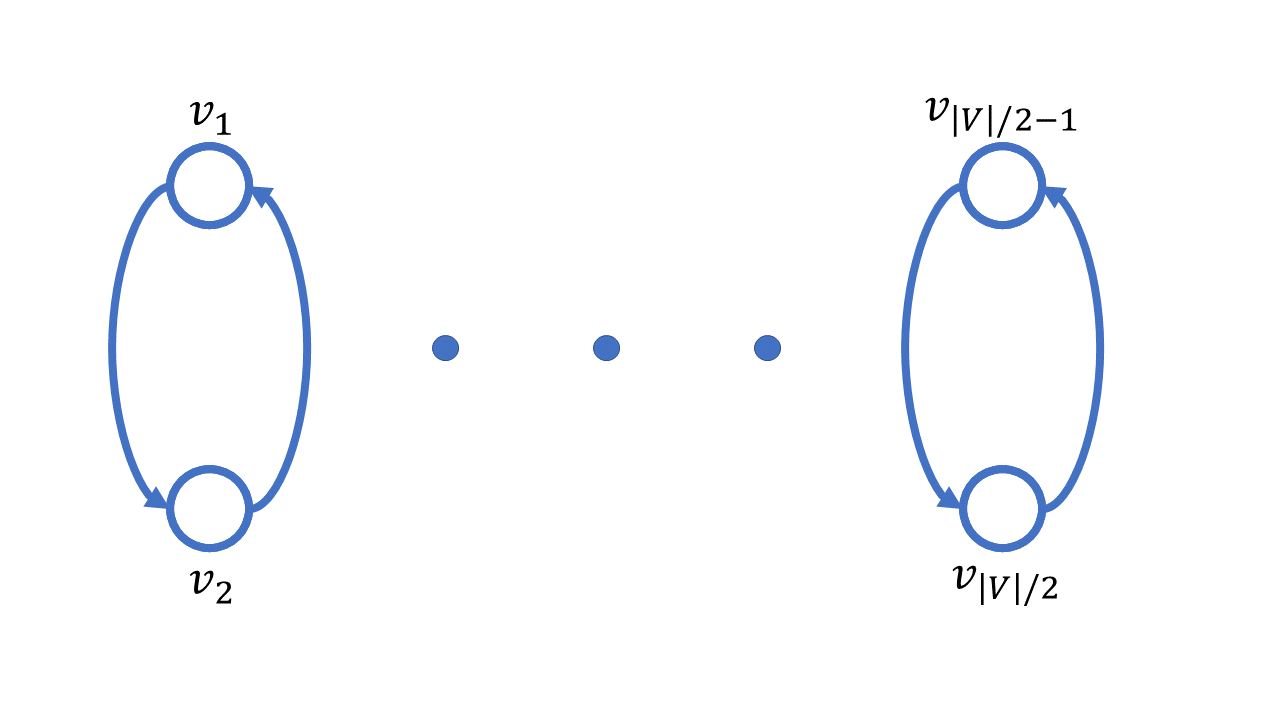
\includegraphics[width=.6\textwidth]{gfx/graph}
\caption{\label{fig:graph} Graph which achieves the bound given in Theorem~\ref{thm:main}.}
\end{figure}

\bibliographystyle{ieeetr}
\bibliography{../../library/library}





%\begin{figure}
%%\centerline{\includegraphics[scale=0.35]{gfx/}}
%%\vspace{-1em}
%\caption{Here's a figure caption!}
%\label{fig:}
%%\vspace{-5mm}
%\end{figure}


\end{document}


